Selain keselamatan dan efisiensi navigasi, kualitas pergerakan robot juga menjadi aspek penting dalam evaluasi sistem navigasi otonom. Robot yang mampu mencapai tujuan dengan aman belum tentu menghasilkan pergerakan yang stabil apabila selama proses navigasi terjadi perubahan arah yang berlebihan, osilasi, atau manuver yang tidak diperlukan. Oleh karena itu, penelitian ini juga mengevaluasi karakteristik pergerakan robot menggunakan indikator kehalusan (\textit{smoothness}) yang diperoleh dari kecepatan angular selama navigasi berlangsung.

Pada penelitian ini, kehalusan pergerakan dievaluasi menggunakan nilai rata-rata kecepat\-an angular (\textit{average angular velocity}). Nilai ini menggambarkan intensitas perubahan orientasi robot selama bergerak menuju tujuan. Semakin tinggi nilai kecepatan angular, semakin sering robot melakukan manuver belok atau koreksi arah. Sebaliknya, nilai yang lebih rendah menunjukkan pergerakan yang lebih stabil dan halus.

\subsection{Distribusi Kecepatan Angular}

Distribusi kecepatan angular pada seluruh skenario pengujian ditunjukkan pada Gambar~\ref{fig:smoothness_boxplot}.

\begin{figure}[H]
\centering
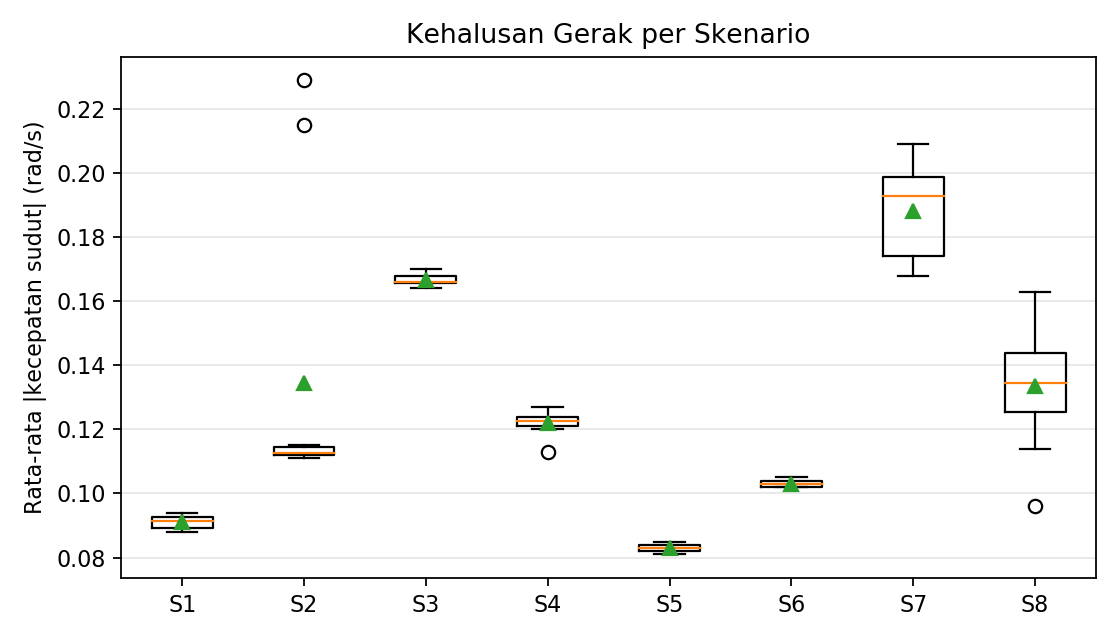
\includegraphics[width=0.75\textwidth]{gambar/fig_smoothness_box.png}
\caption{Distribusi rata-rata kecepatan angular pada seluruh skenario pengujian.}
\label{fig:smoothness_boxplot}
\end{figure}

Secara umum terlihat bahwa nilai kecepatan angular meningkat seiring bertambahnya kompleksitas lingkungan. Pada skenario tanpa obstacle, robot bergerak relatif lurus menuju tujuan sehingga hanya memerlukan sedikit koreksi arah. Ketika obstacle mulai muncul pada jalur navigasi, robot harus melakukan manuver penghindaran yang menyebabkan peningkatan kecepatan angular.

Perbedaan yang lebih jelas terlihat pada pasangan skenario yang melibatkan obstacle berp\-rofil rendah dan obstacle dinamis. Pada konfigurasi baseline, robot cenderung melakukan perubahan arah yang lebih mendadak ketika obstacle berada pada jarak yang dekat. Kondisi tersebut menyebabkan variasi kecepatan angular yang lebih besar selama navigasi berlangsung.

Sebaliknya, konfigurasi fuzzy menunjukkan distribusi kecepatan angular yang lebih terkendali. Meskipun robot melakukan manuver penghindaran yang lebih awal dan mempertahankan jarak aman yang lebih besar terhadap obstacle, perubahan orientasi yang terjadi cenderung lebih bertahap. Hal ini menunjukkan bahwa pengendali fuzzy mampu menghasilkan respons navigasi yang lebih halus dibandingkan konfigurasi baseline.

\subsection{Pengaruh Fuzzy terhadap Kehalusan Navigasi}

Peningkatan kehalusan pergerakan pada konfigurasi fuzzy berkaitan langsung dengan me\-kanisme adaptasi parameter yang diterapkan pada APFPlanner. Ketika obstacle terdeteksi pada jarak dekat atau nilai traversability lingkungan menurun, sistem fuzzy tidak hanya meningkatk\-an penguatan gaya tolak (\textit{repulsive gain}), tetapi juga menurunkan skala kecepatan robot secara bertahap.

Pendekatan tersebut menyebabkan robot mulai melakukan manuver penghindaran sebelum memasuki kondisi yang berisiko tinggi. Akibatnya, perubahan arah yang dilakukan menjadi lebih gradual dibandingkan konfigurasi baseline yang menggunakan parameter tetap. Dengan kata lain, robot tidak perlu melakukan koreksi arah yang agresif karena proses penghindaran obstacle telah dimulai lebih awal.

Karakteristik tersebut juga konsisten dengan hasil yang diperoleh pada Subbab~4.4 dan Subbab~4.5. Peningkatan \textit{minimum clearance} menunjukkan bahwa robot mempertahankan jarak aman yang lebih besar terhadap obstacle, sedangkan peningkatan waktu tempuh menunjukkan bahwa robot bergerak lebih konservatif. Kedua efek tersebut berkontribusi terhadap terbentuknya pola navigasi yang lebih stabil dan lebih halus selama perjalanan menuju tujuan.

\subsection{Implikasi terhadap Stabilitas Sistem Navigasi}

Dari sudut pandang navigasi robot bergerak, pergerakan yang lebih halus memiliki beberapa keuntungan. Pertama, osilasi yang lebih kecil mengurangi kemungkinan robot memasuki kondisi lokal yang tidak stabil ketika berinteraksi dengan obstacle. Kedua, perubahan arah yang lebih gradual menghasilkan lintasan yang lebih mudah diprediksi. Ketiga, perilaku navigasi yang lebih stabil berpotensi meningkatkan kenyamanan dan keamanan apabila sistem diterapkan pada lingkungan yang melibatkan interaksi dengan manusia.

Hasil pengujian menunjukkan bahwa integrasi kamera termal dan pengendali fuzzy tidak hanya meningkatkan keselamatan navigasi melalui peningkatan \textit{minimum clearance}, tetapi juga menghasilkan perilaku navigasi yang lebih stabil. Dengan demikian, manfaat metode yang diusulkan tidak terbatas pada kemampuan menghindari obstacle, tetapi juga mencakup peningkatan kualitas pergerakan robot secara keseluruhan.
